\section{Zufallsvariable und Erwartungswert}

\subsection[Zufallsvariable]{Zufallsvariable $\bm{X}$}

Die Zufallsvariable $X$ ist eine Funktion $X: \, \Omega \rightarrow \mathbb{R}$ , die einem Versuchsausgang $\omega$ einen Wert
$X(\omega)$ zuordnet. \\
\textrightarrow\ Ein Wert, der vom Ausgang eines Zufallsexperiments abhängt

\vspace{0.2cm}

Die Zufälligkeit liegt in dem Versuch, der das $\omega$ ermittelt. \\
Die Zuweisung des Wertes $X(\omega)$ ist \textbf{deterministisch}


\subsubsection{Diskrete Zufallsvariable}

\begin{minipage}[c]{0.58\columnwidth}
	\raggedright
	Eine Zufallsvariable heisst \textbf{diskret}, wenn sie nur \textbf{einzelne genau bestimmte Zahlenwerte}
	$x_1, \, x_2, \, x_3, \, ...$ annehmen kann
	
	\vspace{0.2cm}

	Beispiel: Würfel 
\end{minipage}
\hfill
\begin{minipage}[c]{0.4\columnwidth}
	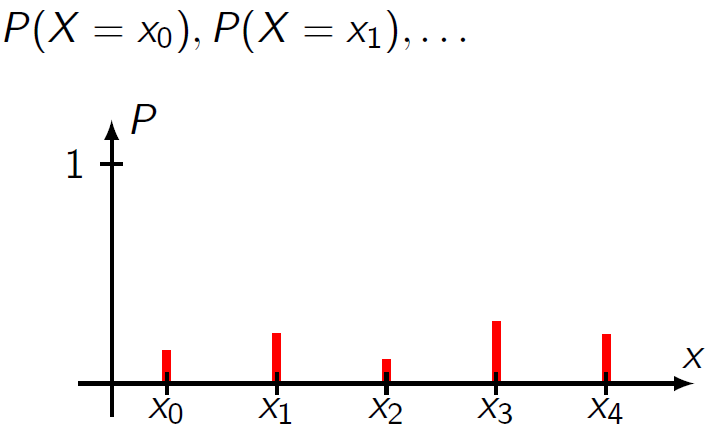
\includegraphics[width=\columnwidth]{images/wahrscheinlichkeit_diskrete_zufallsvariable.png}
\end{minipage}



\subsubsection{Stetige Zufallsvariable}


\begin{minipage}[c]{0.58\columnwidth}
	\raggedright
	Eine Zufallsvariable heisst \textbf{stetig}, wenn sie \textbf{beliebige Werte in einem Intervall} 
	annehmen kann (Wertemenge ist nicht diskret)

	\vspace{0.2cm}

	Beispiel: Messwerte
\end{minipage}
\hfill
\begin{minipage}[c]{0.4\columnwidth}
	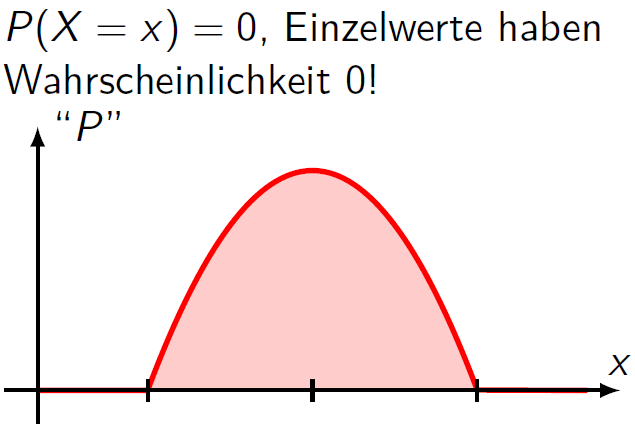
\includegraphics[width=\columnwidth]{images/wahrscheinlichkeit_stetige_zufallsvariable.png}
\end{minipage}




\subsubsection{Notation}

\myul{\textbf{Ereignisse}}

\vspace{0.1cm}

Die Zufallsvariable $X$ definiert neue Ereignisse \\
$A = \{ X \leq a  \} = \{ \omega \in \Omega | X(\omega) \leq a \}$ 

\vspace{0.2cm}

\myul{\textbf{Wahrscheinlichkeiten}}

\vspace{0.1cm}

$P(X = a) = P( \{ X \leq a  \}) = P( \{ \omega \in \Omega | X(\omega) \leq a \} )$ 



\subsection[Erwartungswert]{Erwartungswert  $\bm{E(X)}$} 

Ist $X$ eine Zufallsvariable, dann ist der Erwartungswert
$$  \boxed{ E(X) =\sum \text{Wert} \cdot \text{Wahrscheinlichkeit} } $$
$$ E(X) = \sum\limits_{\omega \in \Omega} X(\omega) \cdot P(\{ \omega \} ) = \sum\limits_{i=1}^k X(A_i) \cdot P(A_i)  $$ 
wobei $X$ konstant auf $A_i$ und $\cup \, A_i = \Omega$ sein muss.


\subsection{Empirischer Erwartungswert}

Der Empirische Erwartungswert entspricht einem \textbf{gewichteten Mittelwert} \\
\textrightarrow\ Notenberechnung

\begin{minipage}[c]{0.48\columnwidth}
	$$ P(X = x_i) = \frac{n_i}{n} $$
\end{minipage}
\hfill
\begin{minipage}[c]{0.48\columnwidth}
	\begin{tabular}{ll}
		$n_i$	& Gewichtung 		\\
		$n$ 	& Anzahl Messwerte
	\end{tabular}
\end{minipage}

\vspace{0.2cm}

$$ \boxed{ E(X) = \sum\limits_i X(i) \cdot P(X = x_i) \approx \sum\limits_i x_i \cdot \frac{n_i}{n} = \frac{x_1 n_1 + ... + x_k n_k}{n} } $$


\subsection{Rechenregeln Erwartungswert}

\textbf{Intuition:} Rechenregeln vom Differenzieren / Integrieren funktionieren auch für den Erwartungswert!


\subsubsection{Multiplikation mit Konstante}

\vspace{-0.2cm}
$$ \boxed{ E( \cor{\lambda} \, X) = \sum\limits_{\omega} \cor{\lambda} \, X(\omega) \cdot P(\omega) = \cor{\lambda} \cdot E(X) } $$


\subsubsection{Erwartungswert einer Konstanten $a$}

\vspace{-0.2cm}
$$ \boxed{ E(a) = a } $$


\subsubsection{Erwartungswert vom Erwartungswert}

\vspace{-0.2cm}
$$ \boxed{ E(E(X)) = E(X) } $$


\subsubsection{Summen}

\vspace{-0.2cm}
$$ \boxed{ E(X + Y) = E(X) + E(Y) } $$

\vspace{0.2cm}

\myul{\textbf{Herleitung}}

\vspace{0.1cm}

\begin{tabular}{ll}
	$E(X + Y)$	& $= \sum\limits_{\omega} \big( X(\omega) + Y(\omega)  \big) \cdot P(\omega)$ 										\\
				& $= \sum\limits_{\omega} X(\omega) \cdot P(\omega) + \sum\limits_{\omega} Y(\omega) \cdot P(\omega) = E(X) + E(Y)$
\end{tabular}
 

\subsubsection{Verbindung zur Wahrscheinlichkeit}

\textrightarrow\ Es gibt \textbf{nur zwei mögliche Versuchsausgänge}, man gewinnt oder man gewinnt nicht

\vspace{0.2cm}

Ist $ A \subset \Omega$ ein Ereignis, dann ist die \textbf{charakteristische Funktion} $\chi_A$ von $A$ eine Zufallsvariable 
$$ \chi_A: \, \Omega \rightarrow \mathbb{R}: \omega \mapsto \chi_A(\omega) =
\begin{cases} 1 & \omega \in A \\ 0 & \omega \notin A \end{cases} $$
Ihr Erwartungswert ist 
$$ \boxed{ E(\chi_A)= P(A) } $$

\vspace{0.2cm}

\myul{\textbf{Herleitung}}

\vspace{0.1cm}

$ E(\chi_A )=  \chi_A(A) \cdot P(A) + \chi_A(\overline{A}) \cdot P(\overline{A}) = 1 \cdot P(A) + 0 \cdot (1- P(A)) = P(A) $


\subsection{Unabhängigkeit}

$X$ und $Y$ sind unabhängig, wenn die Ereignisse $\{ X \leq x \} $ und $\{ Y \leq y \} $ unabhängig sind.

\vspace{0.2cm}

\begin{minipage}[c]{0.48\columnwidth}
	\begin{center}
		\crd{Bei Unabhängigkeit gilt:}
	\end{center}
	$$ \boxed{ E(XY) = E(X) \cdot E(Y) }$$
\end{minipage}
\hfill
\begin{minipage}[c]{0.48\columnwidth}
	\begin{tabular}{lcl}
		unabhängig		& $\Rightarrow$		& unkorreliert	\\
		unkorreliert 	& $\nRightarrow$ 	& unabhängig
	\end{tabular}
\end{minipage}


\subsection[Varianz]{Varianz $\bm{\var(X)}$}

Die Varianz misst die 'Streuung' einer Zufallsvariable und entspricht der mittleren quadratischen Abweichung vom Erwartungswert. \\
Die Formel gilt auch für empirische Daten (Messwerte)

\begin{minipage}[c]{0.4\columnwidth}
	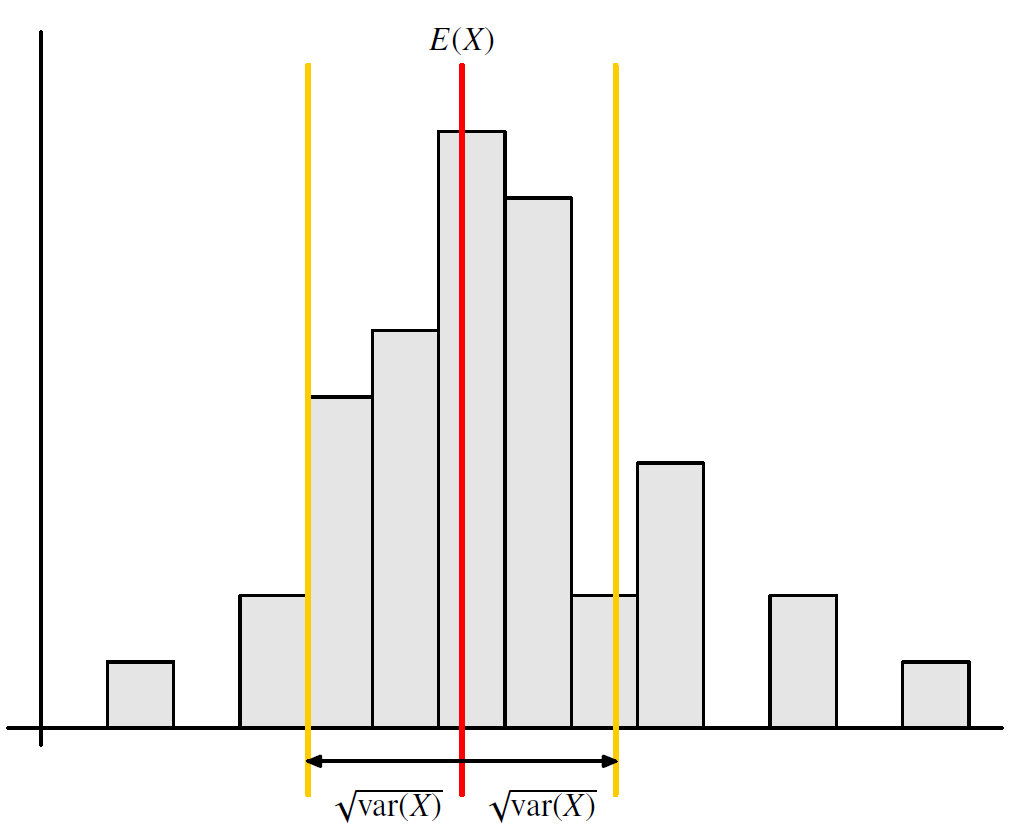
\includegraphics[width=\columnwidth]{images/varianz_darstellung.png}
\end{minipage}
\hfill
\begin{minipage}[c]{0.48\columnwidth}
	$$ \boxed{  \var(X) = E( \, (X - E(X))^2 \, ) }  $$
	$$ \boxed{  \var(X) = E(X^2) - E(X)^2 } $$
\end{minipage}


\subsubsection{Rechenregeln Varianz}

\crd{Für \textbf{unabhängige} Zufallsvariablen} $X$ und $Y$ gilt:

\vspace{0.2cm}

\begin{minipage}[c]{0.48\columnwidth}
	$$ \boxed{  \var(\lambda \, X) = \lambda^{\crd{2}} \var(X) } $$
\end{minipage}
\hfill
\begin{minipage}[c]{0.48\columnwidth}
	$$ \boxed{  \var(X + Y) = \var(X)+ \var(Y) } $$
\end{minipage}


\subsection[Kovazianz]{Kovazianz $\cov(X, \, Y)$}

Die Kovarianz ist ein Korrelationsmass für $X$ und $Y$ 
$$ \boxed{ \cov(X, \, Y) = E(XY) - E(X) \cdot E(Y) } $$


\subsection{Tschebyscheff-Ungleichung}

\textbf{Wahrscheinlichkeit, ausserhalb der Toleranz zu landen} \\
Ist $X$ eine Zufallsvariable mit Erwartungswert $\mu = E(X)$, dann gilt:

\vspace{0.2cm}

\begin{minipage}{0.48\columnwidth}
	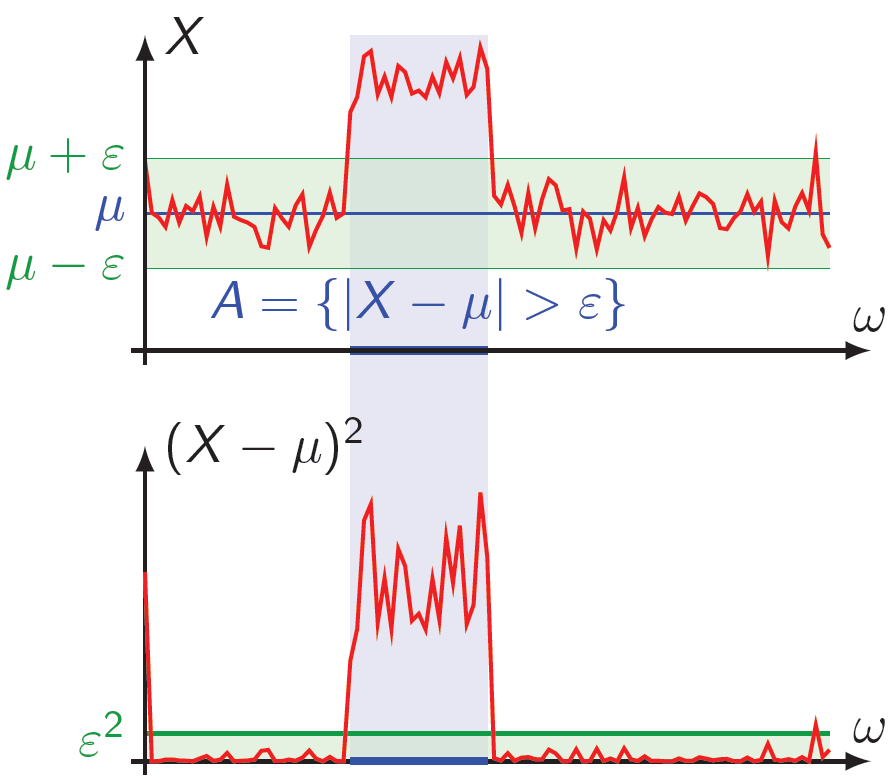
\includegraphics[width=\columnwidth]{images/tschebyscheff_ungleichung.png}
\end{minipage}
\hfill
\begin{minipage}{0.48\columnwidth}
	$$ \boxed{ P( | \crd{X} - \mu | > \varepsilon ) \leq \frac{\var(X)}{\varepsilon^2} = A } $$
	
	\vspace{0.2cm}

	\textrightarrow\ Wenn die Streubreite (Varianz) zunimmt, nimmt auch die Wahrscheinlichkeit zu, ausserhalb der 'Toleranz' zu landen
\end{minipage}


\subsection{Bernoulli: Genauigkeit des Mittelwertes}

\textbf{Abweichung des Mittelwerts vom Erwartungswert}

Gegeben: Zufallsvariable $X$ \\
Stichproben: $X_1, \, \ldots \, X_n$ Zufallsvariablen mit gleichem \\
Erwartungswert $\mu = E(X) = E(X_1) = \ldots = E(X_n)$ und gleicher \\
Varianz $\var(X) = \var(X_1) = \ldots = \var(X_n)$

\vspace{0.1cm}

$M_n = \frac{X_1 + \ldots + X_n}{n}$ \qquad $E(M_n) = E(X)$ \qquad $\var(M_n) = \frac{1}{n} \var(X)$
$$ \boxed{ P( | M_n - \mu | > \varepsilon ) \leq \frac{\var(X)}{ n \cdot \varepsilon^2} } $$

\textrightarrow\ Je mehr Messungen, desto unwahrscheinlicher eine grosse Abweichung des Mittelwerts vom Erwartungswert 


\subsection{Bernoulli: Gesetz der grossen Zahlen}

\textbf{Abweichung relative Häufigkeit von der Wahrscheinlichkeit} 

Ereignis: $A \subset \Omega$ \\
Experiment: $X = \chi_A$, Werte \{0,1\}, $P(A) = E(X)$, $\var(X) = P(A) - P(A)^2 = P(A)(1- P(A))$ 

\vspace{0.1cm}

Wiederholtes Experiment: $X_1, \, ..., \, X_n$, Stichprobe von $X$

\vspace{0.1cm}

Relative Häufigkeit: $h_n = \frac{X_1, \, ..., \, X_n}{n}$, $E(h_n) = P(A)$ \\
$\var(h_n) = \frac{1}{n} \var(X) = \frac{1}{n} P(A)(1-P(A))$ 

$$ \boxed{ P( | h_n - P(A) | > \varepsilon ) \leq \frac{P(A)(1-P(A))}{ n \cdot \varepsilon^2} \leq \frac{1}{4 \, n \, \varepsilon^2} } $$

\textrightarrow\ Je grösser die Anzahl Durchführungen $n$, desto kleiner die Wahrscheinlichkeit, dass die relative Häufigkeit 
stark von der Wahrscheilichkeit abweicht.


\subsection{Lineare Regression (Vorlage!)}

Ein Set von Messwerten $(x, \, y)$ soll mit einer \textbf{Geraden} $y = \cbl{a} \cdot x + \cbl{b}$ \textbf{approximiert} werden. 
Dabei sollen die Parameter $\cbl{a}$ und $\cbl{b}$ der Geraden so bestimmt werden, dass der \textbf{Fehler  $\var(Y-aX-b)$ \\ 
der Approximation minimal} wird.

\vspace{0.2cm}

\textrightarrow\ Entspricht 'Least Squares' Verfahren aus der Linearen Algebra 

$$  \boxed{ \cbl{a} = \frac{E(XY) - E(X) E(Y)}{E(X^2) - E(X)^2} = \frac{\cov(X,Y)}{\var(X)} } $$
$$  \boxed{ \cbl{b} = E(Y) - \cbl{a}  E(X) } $$


\subsubsection{Fehlerberechnung der Approximation}

\myul{\textbf{Fehler $\bm{Z}$}}
$$ \boxed{ Z = \var(Y) \Big( 1 - \frac{\cov(X,Y)^2}{\var(X) \, \var(Y)} \Big) = \var(Y)(1-r^2) } $$ 

\vspace{0.2cm}

\myul{\textbf{Regressionskoeffizient $r$}}
$$ \boxed{ r = \frac{\cov(X, Y)}{\sqrt{\var(X) \cdot \var(Y)}} } $$

\textrightarrow\ Der Fehler $Z$ wird klein, wenn $r^2$ nahe bei $1$ ist, also $r$ nahe bei $\pm 1$


\subsection{Nichtlineare Regression}

Mit einigen 'Umwandlungs-Tricks' können auch einige nichtlineare Funktionen linear gemacht werden und somit wieder
linear approximiert werden

\begin{center}
	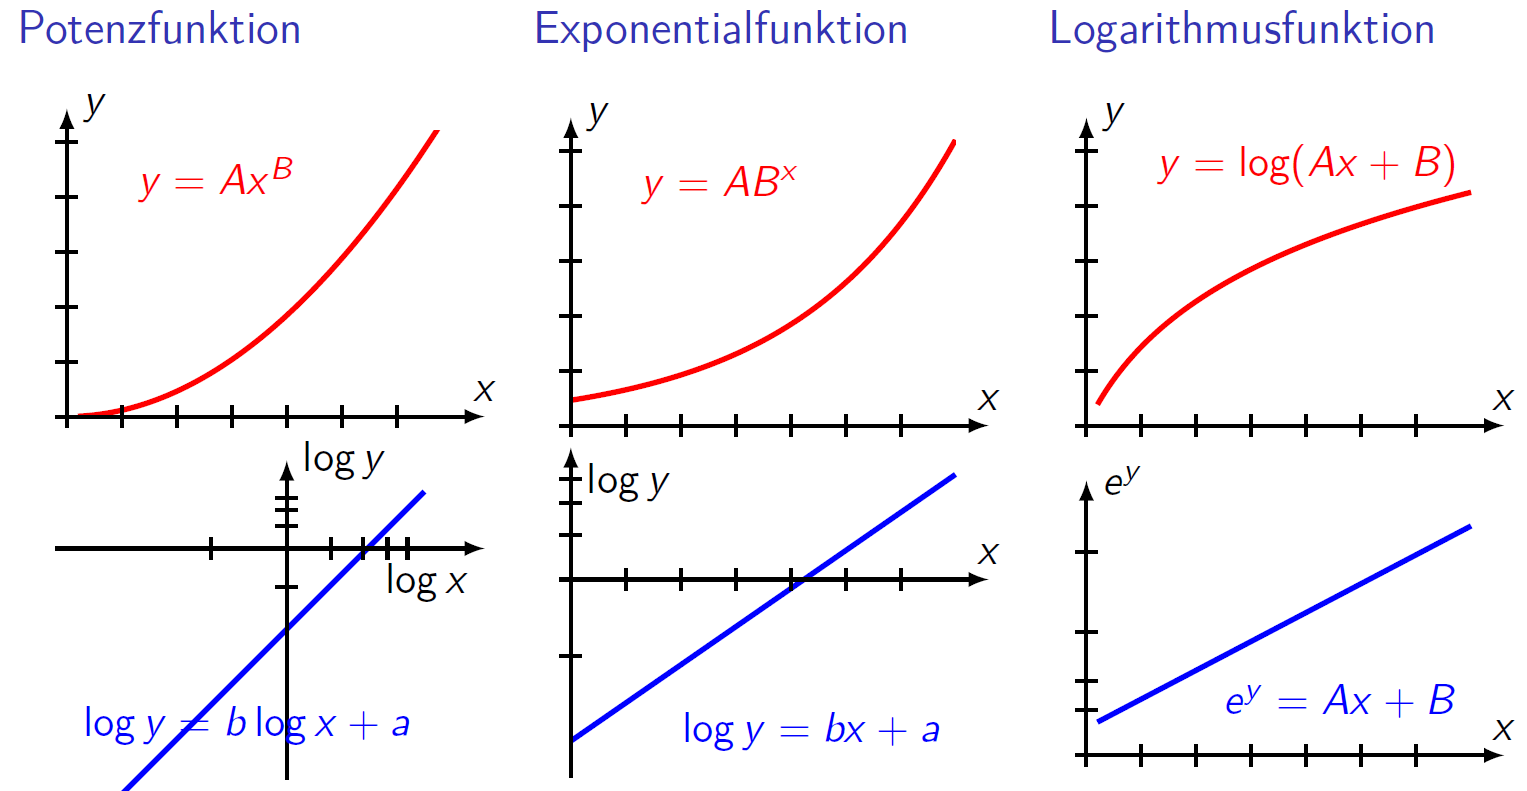
\includegraphics[width=0.8\columnwidth]{images/nichtlineare_regression.png}
\end{center}

\begin{tabular}{l c l}
	$y = Ax^B$			& \textrightarrow\	& $\log(y) = b \log(x) + \log(a)$ 	\\
						& \textrightarrow\ 	& $X = \log(x)$ ; $Y = \log(y)$ 	\\
	\\	
	$y = AB^x$ 			& \textrightarrow\ 	& $\log(y) = x (\log(B)) + \log(A)$ \\
						& \textrightarrow\ 	& $X = x$ ; $Y = \log(y)$ 			\\
	\\		
	$y = \log(Ax +B)$ 	& \textrightarrow\ 	& $e^y = Ax + B $					\\
						& \textrightarrow\ 	& $X = x$ ; $Y = e^y$
\end{tabular}

